\documentclass{aicom2e}
\usepackage{amsmath}
\interdisplaylinepenalty=2500
\usepackage[algo2e,ruled,vlined,linesnumbered]{algorithm2e}
\usepackage[active]{srcltx}


\usepackage{amsthm, amssymb,amsfonts}
\usepackage{graphicx}
\usepackage{epsfig}
\usepackage{latexsym}
\usepackage{colortbl}
\usepackage{times}
\usepackage{helvet}
\usepackage{courier}
\usepackage{caption}
\usepackage{subfig}
\usepackage{float}
\usepackage{xcolor}
\usepackage{pslatex}
\usepackage{eso-pic}
\usepackage[bottom]{footmisc}
\usepackage{url}
\usepackage{etex}


\newtheorem{definition}{Definition}
\newtheorem{lemma}{Lemma}
\newtheorem{theorem}{Theorem}
\newtheorem{observation}{Observation}
\newcommand{\kgs}{$k$-goal search}
\newcommand{\kgbfs}{$k$-goal best-first search}


\newcommand{\astar}{A$^*$}
\newcommand{\kastar}{kA$^*$}
\newcommand{\kastarmin}{kA$^*_{min}$}
\newcommand{\kastarmax}{kA$^*_{max}$}
\newcommand{\kxastar}{k$\times$A$^*$}
\newcommand{\astari}[1]{A[$#1$]}

\newcommand{\minf}{Min-f}
\newcommand{\maxf}{Max-f}
\newcommand{\tuple}[1]{\ensuremath{\left \langle #1 \right \rangle }}
\newcommand{\open}{\textsc{Open}}
\newcommand{\closed}{\textsc{Closed}}
\DeclareMathOperator*{\argmin}{\arg\!\min}
\newcommand{\roni}[1]{\textbf{[RS:#1]}}
%\newenvironment{proof}{\noindent{\bf Proof:~~}}{\qed}

\begin{document}
\begin{frontmatter}                           % The preamble begins here.
%
%\pretitle{Pretitle}
\title{Shortest Path for K Goals}
% \runningtitle{Running title}
%\subtitle{Subtitle}
\maketitle
%
\author[]{Ariel Felner}
\address{Ben Gurion University of the Negev\\ Be'er Sheva, Israel\\
    E-mail: felner@bgu.ac.il}

\author[]{Meir Goldenberg}
\address{The Jerusalem College of Technology\\ Jerusalem, Israel\\
    E-mail: mgoldenbe@gmail.com}
\author[]{Roni Stern}
\address{Ben Gurion University of the Negev\\ Be'er Sheva, Israel\\
    E-mail: roni.stern@gmail.com}

\begin{abstract}
Abstract...

\end{abstract}

\begin{keyword}
artificial intelligence\sep AI\sep Heuristic Search
\end{keyword}
%
\end{frontmatter}

\section*{Introduction}


The shortest path problem (SSP) in a graph is the problem of finding the lowest cost path in a graph from one vertex -- denoted the {\em start} vertex -- to another vertex -- denoted the {\em goal} vertex.
SSP is a well-studied problem and many algorithms have been proposed for solving it.
Many times SPP is activated on explicitly given graphs such as roadmaps, grids, planning for robots and game maps~\cite{Ststurtevant2012benchmarks}. 

Now, imagine $k$ SSP problems, such that all the problems share the same start vertex.
Solving this set of SSP problems is called the $k$-goal problem.
A trivial solution to \kgs\ is to run a SSP solver $k$ times. Alternatively,
we can construct a $k$-dimensional SSP problem, and try to solve all the $k$ SSP problems concurrently.
In this work we study the interplay between these two extreme approaches and
study how heuristics can be used correctly to solve \kgs.


\roni{TODO: SOME RELATED WORK?}

\section{Background and Problem Definition}

%In this section, we formally define the $k$-goal search problem.

% Graphs, costs, SSP
Let $G=(V,E,w)$ be a weighted graph, where $V$ is the set of vertices, $E$ is the set of edges, and $w:E\rightarrow \mathbb{R}^+$ is a function that assigns a non-negative real value to each edge. This value is referred to as the {\em cost} of the edge. The cost of a path in a graph is the sum the edge costs along it. 
In the Artificial Intelligence literature, graphs are often used to represent state spaces, 
where the graph vertices represent possible states of the world, the out-going edges of a vertex represent possible actions that an agent can perform in the corresponding state, and the cost of an edge represents the cost of the corresponding action. 
Thus, throughout this paper we will use the terms {\em states} and {\em actions} instead of vertices and edges, respectively, and use the term {\em applying an action} instead of traversing an edge. Note that a path in a graph corresponds to an applicable sequence of actions. 

\begin{definition}[The Shortest Path Problem (SPP)]
A shortest path problem (SPP) is defined by a tuple $\tuple{G,s,g}$, where $s$
and $g$ are states in $G$ and the problem is to find the lowest cost path in
$G$ from $s$ to $g$. \label{def:spp}
\end{definition}

\subsection{The \astar{} Algorithm}




\begin{algorithm2e}[t!]
	\small
	\KwIn{Start state $s$, Goal state $g$)}
	$g(s)\gets 0$; \open{}~$\gets\emptyset$; \closed{}~$\gets \emptyset$\\
	Add $s$ to \open{} with $f(s)=g(s)+h(s)$\\
	\While {\open{} $\neq \emptyset$} {
		$n \gets \argmin\limits_{n\in\open{}} f(n)$ \nllabel{line:open:chooseNode}\\
		Move $n$ from \open{} to \closed{}\\
		\lIf {$n$ is the goal}{\Return the best path found to $n$}
		\For{every action $A$ applicable at state $n$ \nllabel{line:nextNeighbor}}{
			$c \gets $ generate a state by applying $A$ to $n$ \nllabel{line:astar:generate-start}\\			
			
			% Duplicate detection
			\If{$c$ in $\open{}\cup \closed{}$ \nllabel{line:dd-start}}{
				\If{$g(c) \leq g(n)+w((n,c))$}{
					{\bf continue} (goto line~\ref{line:nextNeighbor})
				}
				Remove $c$ from \open{} and \closed{}  \nllabel{line:dd-end}\\
			}
			% Update n's g and f values
			$g(c)\gets g(n)+w((n,c))$ \nllabel{line:compute-f}\\ 							
			Add $c$ to \open{} with $f(c)=g(c)+h(c)$  \nllabel{line:astar:generate-end}\\
		}
	}
	\Return No solution exists\\ 
	\caption{\astar{}}
	\label{alg:astar}
\end{algorithm2e}



% A* for single agent search
SPP has been well-studied in the literature. \astar{}~\cite{hartNR68Astar} is a popular 
heuristic search algorithm for solving SPP. For completeness, we provide below a short description of \astar{} and Algorithm~\ref{alg:astar} presents its pseudo-code. 
\astar{} maintains two lists of states: \open{} and \closed{}. 
Initially, \closed{} is empty and \open{} contains only the start state ($s$). 
Every state that is added to \open{} is associated with a $g$ value and an $f$ value. 
The $g$ value of a state $n$, denoted $g(n)$, is the cost of the lowest cost path found so far from the start state $s$ to $n$. Hence, $g(s)$ is set to zero. 
The $f$ value of $n$, denoted $f(n)$ is the sum of $g(n)$ and a heuristic estimate of the cost of the lowest cost path from $n$ to the goal state $g$. 
This heuristic estimate is denoted by $h(n)$, and there is an abundance of prior work in the literature on how to develop effective heuristics. \roni{TODO: Add some refs here}


In every iteration of \astar{}, the state with the lowest $f$ value in \open{} is moved from \open{} to \closed{}. 
If that state is a goal, the search halts returning the path found to it.\footnote{We omit in this pseudo code how back-pointers are maintained to  preserve the best path to each state.} Otherwise, the state is {\em expanded}.  
Expanding a state $n$ means generating every state that can be reached by applying a single action at state $n$. 
Then, the $g$ and $f$ values of every generated state $c$ are computed based on the $g$ value of its parent, the cost of the action used to generate $c$, and the heuristic estimate $h(c)$. Finally, the generated states are added to \open{} with their $f$ values, to be considered for expansion in future iterations. Since the searched graph may not be a tree, multiple paths to the same state may be explored, and \astar{} keeps track of only the best (lowest cost) path it finds to every generated state (lines~\ref{line:dd-start}-\ref{line:dd-end}).  


\roni{TODO: Maybe add more line numbers to the text?}
\roni{TODO: Add something on tie breaking}

% A* properties and admissible heursitics
\astar{} has several important properties. First, if the heuristic used is {\em admissible}, i.e., it does not over-estimate the cost of the lowest cost path to the goal, then \astar{} is guaranteed to solve SPP, i.e., to return a lowest cost path from $s$ to $g$.\footnote{In fact, it is sufficient that the heuristic is admissible only for the states that are on a single lowest-cost path for \astar{} to guarantee optimality~\cite{karpas2012optimal,dechter1985generalizedBestFirst}.} 
Second, if the heuristic is {\em consistent} then \astar{} is guaranteed to never expand a state more than once. 
%when a state $n$ is expanded it is guaranteed that the lowest cost path from $s$ to $n$ has been found, and thus $g(n)$ is the cost lowest cost path from $s$ to $n$. 
\begin{definition}[Consistent Heuristic~\cite{hartNR68Astar}]
    A heuristic $h$ is {\bf consistent} if for every pair of states $x$ and $y$
    it holds that $h(x)\leq d(x,y)+h(y)$, where $d(x, y)$ is
    the cost of the lowest-cost path from $x$ to $y$.
    \label{def:consistent}
\end{definition}



%The important implication of a consistent heuristic is that \astar{} with a consistent heuristic is guaranteed to expand every state at most once. 
Third, under some conditions, it can be shown that up to tie-breaking between states with equal $f$ values, \astar{} will only expand the minimal set of states required to find an optimal solution~\cite{dechter1985generalizedBestFirst}. 
A recent variant of \astar{} provides a similar guarantee with respect to the number of states generated as well~\cite{goldenberg2014enhanced}. This type of guarantees, often referred to as the {\em optimally effective} property of \astar{}, is  important because in many cases the runtime of the algorithm is correlated with the number of states expanded/generated. 
Thus, guaranteeing that \astar{} expands/generates the minimal number of states provides some sort of optimality guarantee for \astar{}'s efficiency compared to other equally informed algorithms. 



\subsection{The $k$-Goal Problem}
In this paper we focus on the $k$-goal search problem, which can be viewed as a generalization of SPP. 

In this paper we focus on the $k$-goal search problem, which can be viewed as a
generalization of SPP.

%\begin{definition}[$k$-goal search]
%	A \kgs\ problem is defined by a tuple $\tuple{G,s, g_1, g_2, \ldots, g_k}$, 
%	where $s$ and $g_1, g_2, \ldots, g_k$ are states in $G$ and the problem is to find 
%	$k$ paths $p_1,\ldots p_k$ such that for every $i\in [1,k]$ it holds that $p_i$ is a lowest-cost path from $s$ to $g_i$. 
%	\label{def:k-goal}
%\end{definition}


\begin{definition}[$k$-goal search]
	A \kgs\ problem is defined by a tuple $\tuple{G,s, \textbf{g}}$
		where $G$ is a graph
		$s$ is state in $G$, 
		and $\textbf{g}=(g_1,g_2,\ldots,g_k)$ is a vector of $k$ states. 
	A solution to the \kgs{} problem is a set of $k$ paths $p_1,\ldots p_k$ such that for every 
	$i\in [1,k]$ it holds that $p_i$ is a lowest-cost path from $s$ to $g_i$. 
\label{def:k-goal}
\end{definition}


% k searches independentaly
Clearly, SPP is a special case of \kgs\ with $k=1$. A trivial solution to \kgs\ is to consider it as $k$ independent SPPs and use \astar{} (or any other SPP algorithm) multiple times to solve these $k$ problems. 
In the next section we present this approach and analyze its complexity. In later sections we introduce a different approach that activates a single search that aims to find all $k$ goals concurrently. This allows sharing and re-using information between the $k$ different tasks, potentially decreasing the overall search effort. 




\section{$k$ Searches for One Goal}
\label{sec:k-one-goal}
\begin{algorithm2e}[t!]
	\small
	\KwIn{Start state $s$, Goals vector $\textbf{g}=(g_1,\ldots g_k$)}
	\For{$i$=1 to $k$}{
		$p_i\gets$ \astar{}($s$,$g_i$)\\
	}
	\Return $p_1,\ldots p_k$\\	
	\caption{\kxastar{}: \kgs{} with $k$ \astar{}s}
	\label{alg:k-searches}
\end{algorithm2e}



Algorithm~\ref{alg:k-searches} outlines the trivial approach for solving \kgs{}: running \astar{} $k$ times, one for each of the $k$ goals. The resulting $k$ paths are returned as a solution to the \kgs{} problem. We refer to Algorithm~\ref{alg:k-searches} as \kxastar{}. 


To analyze the effectiveness of \kxastar{}, we use the notions of {\em necessary} states and {\em surplus} states~\cite{goldenberg2014enhanced}. 
%\roni{Meir and Ariel: who used this term before us?}

\begin{definition}[Surplus States and Necessary States]
	Let $\Pi$ be a SPP defined by the tuple $\tuple{G,s,g}$, and let $opt_\Pi$ denote the cost of a solution to $\Pi$. 
	A state $n$ is called a {\em necessary} state with respect to $\Pi$ if $f(n)<opt_\Pi$. 
	A state $n$ is called a {\em surplus} state with respect to $\Pi$ if $f(n)>opt_\Pi$. 
\label{def:surplus}
\end{definition}
Without any additional knowledge of the graph $G$, one needs to expand every necessary state in order to solve a given SPP, 
and one can solve a given SPP without expanding any surplus state. \roni{Meir/Ariel, what would be a good reference to put here? Dechter and Pearl? it is important to be accurate here}
\astar{} must expand all necessary states but will never expand any surplus state. 

Consequently, if $\Pi_i$ is the SPP problem from $s$ to $g_i$ 
then using \kxastar{} to solve \kgs{} will end up expanding every state that is necessary w.r.t at least one of the $k$ SPP problems $\Pi_1,\ldots \Pi_k$ and never expand any state that is surplus w.r.t all these SPP problems. 
Hence, one might think that \kxastar{} is ``optimally effective'' for \kgs{}, 
expanding exactly the set of needs one must expand in order to solve the problem, up to tie-breaking between states with the same $f$ value. 


This conclusion is not accurate, however, as it overlooks two potential sources for improvement:
\begin{itemize}
	\item {\bf Learning from experience.} When solving one SPP problem, e.g., for goal $g_1$, one gains additional knowledge of the searched graph, which may be used when solving the subsequent SPPs for the other goals.
	\item {\bf Avoiding duplicates.} The same state can be generated and expanded in multiple SPPs. For example, using Algorithm~\ref{alg:k-searches} will end up generating the children of the start state at least $k$ times. This introduces redundancy to the search process that may be avoided.  
\end{itemize}
The first source of improvement is related to the literature on incremental search~\cite{koenig2004lifelong} and to moving-target search algorithms~\cite{ishida1995moving,koenig2007speeding}. See Section~\ref{sec:related-work} for details. In this work we focus on this work on the latter source of improvement -- avoiding duplicates. %in the search process. 
%Next, we analyze these redundancies in the search process that are due to such duplicates. 

\subsection{Redundancies in the $k$ Searches Approach}

To analyze the redundant operations performed by \kxastar{}, we first describe the operations performed by \astar{} whenever a state is generated (lines~\ref{line:astar:generate-start}-\ref{line:astar:generate-end} in Algorithm~\ref{alg:astar}):
\begin{enumerate}
\item {\bf Generation}  (line~\ref{line:astar:generate-start}). This means computing the generated state by applying 
an action to the expanded state. This step usually involves setting up some data structure that represents the generated state. If the action generating the state is not too complicated, the complexity of this step is linear in the size of the state. We
denote the computational cost of this step as $C_{gen}$.
\item {\bf Duplicate detection}  (lines~\ref{line:dd-start}-\ref{line:dd-end}). This means performing a lookup in \open{} and \closed{} to see if the generated state was already generated, and if so, whether the current path to it is better than the one previously found. The lookup in \open{} and \closed{} is often implemented by storing all the states that were generated in the past in some hash table and performing an $O(1)$ hash table lookup. We denote the computational cost of this step as $C_{dd}$. 
\item {\bf Heuristic computation}  (line~\ref{line:compute-f}). This means computing the $h$ value of the generated state. Heuristics vary widely in their computational cost, where some heuristics require constant time to compute while more sophisticated heuristics may involve poly-time computations. We denote the computational cost of this step as $C_{h}$. 
\item {\bf Insertion into \open{}}  (line~\ref{line:astar:generate-end}). This means adding a state to \open{} with an associated $f$ value. \open{} are often implemented as a Binary heap or priority queue sorted according to $f$ values, so that extracting the state with lowest $f$ value is very fast. Thus, inserting a state to \open{} may take time that is logarithmic in the size of \open{}. We denote the computational cost of this step as $C_{add}$. In classical heap-based implementation of \open{}, $C_{add}$ is logarithmic in the size of \open{}, but in some cases faster implementations are also possible where adding to \open{} incurs a constant time~\cite{GILON2016,BurnsHLR12}.
\end{enumerate}

%Each of these operations incur some computational cost. Let $C_{gen}, C_{dd}, C_{h},$ and $C_{add}$ denote the average computation cost of the above four operations, generation, duplicate detection, heuristic computation, and insertion into \open{}, respectively. In addition, 

Let \astari{i} denote the \astar{} search used to solve $\Pi_i$, and let $Gen(\astari{i})$ denote the set of states generated by \astari{i}.   
Clearly, \kxastar{} incurs at least $\sum_{i=0}^k |Gen(\astari{i})|\cdot(C_{gen}+C_{dd}+C_{h}+C_{add})$ in terms of computation cost. 
The main source of inefficiency is that the intersection between 
the sets of states generated by the individual \astar{} searches can be not empty. This indicates that there are states will be generated in more than one of the $k$ searches and incurring their overhead ($(C_{gen}+C_{dd}+C_{h}+C_{add})$) more than once.

\begin{figure}
	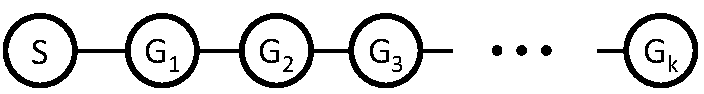
\includegraphics[width=\columnwidth]{k-search-bad_cropped}
	\caption{An example where the $k$ search approach is inefficient.}
	\label{fig:k-search-bad}
\end{figure}
An extreme example of this inefficiency is depicted in Figure~\ref{fig:k-search-bad}. The searched graph is a simple line, 
where $g_1$ is adjacent to $s$, $g_2$ is adjacent to $g_1$, and so on. In this case \kxastar{} would generate
$1+2+3+\cdots+k=\frac{k(k-1)}{2}$ while it is easy to see that generating $k$ states would be sufficient to solve the \kgs{} for this case. 


% Some costs can be saved
However, some of the costs incurred when generating the same state for more than one goal is unavoidable. 
This is because to prove that a path of cost $X$ to a goal $g_i$ is optimal one needs to expand all the necessary states w.r.t $\Pi_i$, 
i.e., generate their children and compute their $f$ values. This is needed to verify that all paths of costs smaller than $X$ have been considered. Since the $f$ value of a state may be different when searching for different goals, this means that a state may be necessary for one search and not necessary for the other. 
Thus, the search must check that $n$ is necessary for each goal independently, incurring a computational cost of $C_{h}$ per goal. 
However, when a state is generated by more than one search there is potential for saving some of the computational costs incurred during its generation. In particular, by generating such states only once, one may save the costs incurred for state generation, duplicate detection, and insertion to \open{} ($C_{gen}, C_{dd},$ and $C_{add}$). In the next section we propose a method for doing so. 


\begin{table*}
	\begin{tabular}{|l|l|}
		\hline
		Gen($X$)	& The set of states generated by algorithm $X$ \\
		Gen$_k(i)$ 	& The number of states generated by \kastar{} until the $i^{th}$ goal is found\\
		Time($X$)	& The runtime required to run algorithm $X$ \\
		$f(n)$		& The state evaluation function used by \astar{}: $f(n)=g(n)+h(n)$ \\
		$F(n)$		& A state evaluation function used by \kastar{} that aggregates a vector of $k$ possibly different $f$ values, one per goal. \\
		$F_{min}$   & $\min_{j\in[1,k] f(n)}$\\
		$F_{max}$   & $\max_{j\in[1,k] f(n)}$\\
		\astari{i}  & An \astar{} for finding the lowest cost path to goal $g_i$. \\
		
		\hline
	\end{tabular}
\label{tab:notations}
\caption{This table summarizes the notations used in this paper.}
\end{table*}


\section{A Single Search for all  $k$ Goals}
\label{sec:one-k-goal-search}
In this section we generalize \astar{} to search for $k$ goals in parallel. 
We call the resulting algorithm \kastar{}. 
Before presenting a complete pseudo code for \kastar{}, we highlight several differences it has from \astar{}. 

\subsubsection*{Multiple heuristics per state.} When a state $n$ is generated, \kastar{} computes 
$k$ different $h$ values for it $\textbf{h}=(h_1(n),\ldots h_k(n))$, where $h_i(n)$ is the heuristic estimate of the cost to get from $n$ to goal $g_i$. These $k$ heuristic values are used to form a $k$-ary vector $\textbf{f}(n)=(f_1(n),\ldots f_k(n))$, where $f_i(n)=g(n)+h_i(n)$. We discuss later how these $k$ $f$-values are aggregated to a single value denoted $F(n)$. \open{} is prioritized according to the $F$ values, i.e., in every iteration we pop from \open{} the state with the lowest $F$ value. Note that the computational effort of generating a state in \kastar{} is larger than that of regular \astar{}, as it requires computing the $k$ heuristics. %computing $F$ costs more than computing an individual $f$ value, as it at least $k\cdot C_h$, and thus the computation cost of generating a state in \kastar{} is larger than that of \astar{} by $(k-1)\cdot C_{h}$.\footnote{As discussed later in the paper, the actual computational cost in \kastar{} can be smaller, since as the search progresses the list of relevant goals becomes smaller, and consequently computing $F$ becomes easier.}

\subsubsection*{Maintaining the active goals.} In \astar{} when a goal is expanded the search halts. By contrast, in \kastar{} the search does not halt until a lowest-cost path to each of the $k$ goals is found. To this end, \kastar{} tracks of the set of goals that were not solved yet, i.e., the goals where the lowest cost path to them has not been found. This set of goals is referred to as the {\em active goals}. Maintaining the list of active goals is also used to avoid redundant heuristic computations: when a state is generated we only compute the heuristics for goals that are still active. 



%\subsubsection*{Node evaluation function.} When searching for a single lowest-cost path with \astar{}, the state are popped from \open{} according to their $f=g+h$ values. In \kastar{}, we compute the $h$-value forand associate every state in \open{} with a value that considers the $h$-value for each of the $k$ goals.     Thus, when a state is generated then we compute the heuristic for each of the $k$ goals.




\begin{algorithm2e}[t!]
	\KwIn{Start state $s$, goal states $g_1,\ldots,g_k$}
	%\SetKwBlock{KGBFS}{$k$-goal best-first-search(start state $s$, goal states $g_1,\ldots,g_k$)}
	\open{}~$\gets\emptyset$ \\
	{\tt ActiveGoals} $\gets \{g_1,\ldots,g_k\}$ \nllabel{line:init-active-goals} \\
	$F\gets$ ComputeF(s, ActiveGoals) \nllabel{line:compute-f-start}\\
	Add $s$ to \open{} with key $F$ \\		
	\While {\open{} $\neq \emptyset$ and {\tt ActiveGoals} not empty} {
		$best \gets$ state in $\open{}$ with the smallest key \nllabel{line:open:chooseNode}\\
		Remove $best$ from \open{}\\
		\If {$best\in$ {\tt ActiveGoalsls}}{
			Add path to $best$ to the solution \nllabel{line:storePath}\\
			Remove $best$ from {\tt ActiveGoals} \nllabel{line:removeGoal}\\
		}
		\For{$n \in neighbors(best)$}{
			$F\gets$ ComputeF(n, {\tt ActiveGoals})\\
			Add $n$ to \open{} with key $F$ \\
		}
	}
	\caption{\kastar{}}
	\label{alg:k-goal-bfs}
\end{algorithm2e}



Algorithm~\ref{alg:k-goal-bfs} shows the pseudo code for \kastar{}. Initially, all goals are inserted into the list of active goals ({\tt RelevantGoals}) [line~\ref{line:init-active-goals} in Alg.~\ref{alg:k-goal-bfs}].  
Every state $n$ that is added to \open{} is associated with a key value $F$ that is computed using the {\tt ComputeF} function. In every iteration, the state with the smallest key value (i.e., minimal $F$ value) is popped out of \open{} (line~\ref{line:open:chooseNode}). If it is a goal then we store the path to it (line~\ref{line:storePath}). In addition, we remove that goal from the {\tt ActiveGoals} list, to mark that we are no longer looking for a path to that goal (line~\ref{line:removeGoal}). When the {\tt ActiveGoals} list is empty, we halt the search, having found a path to each goal. 


It is easy to see that Algorithm~\ref{alg:k-goal-bfs} is complete and sound, in the sense that if there are paths to the $k$-goals they will be found, and the paths returned by the algorithm are all valid paths to the $k$ goals. The key question is whether these paths are indeed the optimal path to the $k$-goals.
As we show next, this depends on the order according to which states are expanded, 
which in turn depends on how $F$ is computed. %)the {\tt ComputeF} function is implemented. 


\subsection{An Evaluation Function for \kastar{}}
In \astar{} for a single goal, states are prioritized in \open{} according to the $f=g+h$ value of a state. 
In contrast, a state in \kastar{} has a vector of $k$ heuristic values $\textbf{h}(n)$ and 
consequently a vector of $f$ values $\textbf{f}$(n) that contains one $f$ value per goal. Therefore, \kastar{} requires a state evaluation function that aggregates these $f$ values in some way. In Algorithm~\ref{alg:k-goal-bfs} this is encapsulated in the {\tt ComputeF} function. We refer to the value ($F$) returned by this function as the state's $F$ value, and consider the following two options for computing it. 
\begin{align}
F_{min}(n)=&\min_{i\in [1,k]}f_i(n) & (\textbf{\minf})\\ 
F_{max}(n)=&\max_{i\in [1,k]}f_i(n) & (\textbf{\maxf}) 
\end{align}
\kastar{} that uses with $F_{min}$ as the state evaluation function ({\tt ComputeF}) 
is referred to hereinafter as \kastarmin{}, and similarly \kastar{} that uses $F_{max}$ is referred to 
as \kastarmax{}.
 

%\subsection{$F_{min}$}

\begin{theorem}[\kastarmin{} is admissible]
If $h$ is an admissible heuristic, then running \kastarmin{} returns $k$ paths
$\pi_1,\ldots, \pi_k$ such that for every $i$ we have that $\pi_i$ is a lowest cost
path from $s$ to $g_i$. \label{the:min-f}
\end{theorem}
 \begin{proof}
To prove this, we show that when a goal state is expanded for the first time,
then its $g$-value is guaranteed to be the cost of the lowest-cost path from
$s$ to that goal. By negation, assume that a goal $g_i$ was expanded, but there
is a better path to $g_i$ that has not yet been discovered. Since \kastar{} is
a best-first search, \open{} has some state $n$ that is on a better path to
$g_i$ and has not been expanded yet. That is,
\begin{equation}
g(n)+h_i(n)<g(g_i)
\label{eq:proof-1}
\end{equation}
Since $g_i$ was chosen to be expanded before $n$, it must have a $F_{min}$ value no-larger than $n$, i.e.,
\begin{align}
F_{min}(n) &\geq  F_{min}(g_i)\\
g(n)+\min_{j\in [1,k]}(h_j(n))& \geq  g(g_i)+\min_{j'\in [1,k]}(h_j(g_i))\\
g(n)+\min_{j\in [1,k]}(h_j(n))& \geq  g(g_i)\\
g(n)+h_i(n) &\geq  g(g_i)
\end{align}
The last line above contradicts Equation~\ref{eq:proof-1}.
\end{proof}


%\subsection{$F_{max}$}
 
 \begin{figure}
 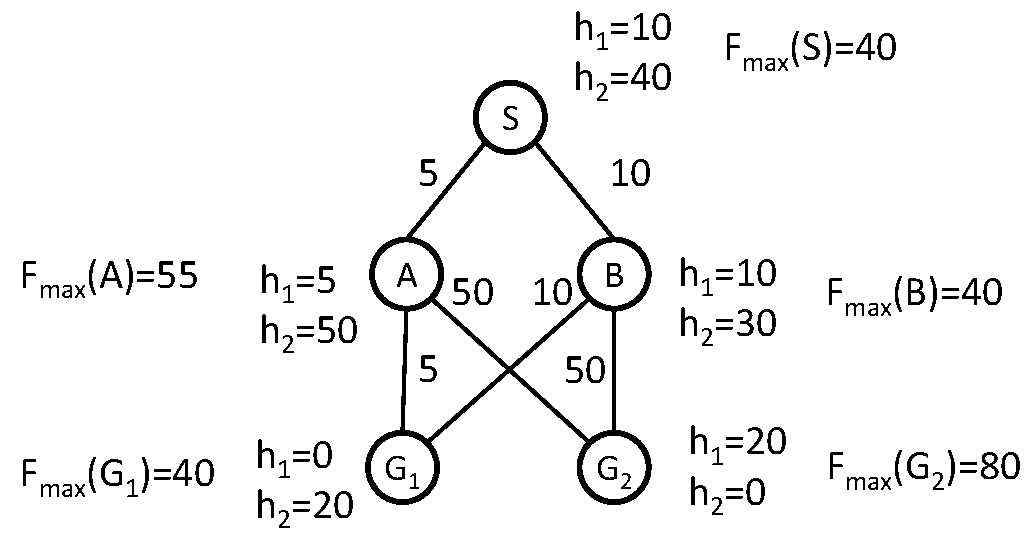
\includegraphics[width=\columnwidth]{max-bad_cropped.pdf}      
 \caption{An example of where using \kastarmax{} returns a non-optimal solution. In this example, 
 using Max-$f$ will results in the following expansion order: $S$, $B$, $g_1$. 
 Thus, when $g_1$ is expanded, the best path known to it costs 25, while a 
 better path to it goes through $A$ and costs only 10.}
 \label{fig:max-bad}
 \end{figure}
 
 \begin{observation}[\kastarmin{} is not admissible]
 	Even if $h$ is an admissible heuristic, 
 	running \kastarmax{} may return a path $\pi_i$ from $s$ to $g_i$ that is not optimal. 
 	\label{obs:max-f-inadmissible}
 \end{observation}
[[AF: overload of terms. $F_{min}(n)$ and \minf{}]]\roni{I don't understand. It's the same term}

To demonstrate Observation~\ref{obs:max-f-inadmissible}, consider the graph in Figure~\ref{fig:max-bad}.
 In this example, using \maxf{} will result in the following expansion order: $S$, $B$, and then $g_1$. At this stage, we expanded one of the goals -- $g_1$ -- while the best path found so far to it goes through $B$ and costs 40. However, a better path to it is through $A$, which costs only 10.
 
 
 % MAX-F is OK for consistent heuristics
  The observant reader may have noticed that the heuristic function in Figure~\ref{fig:max-bad} is inconsistent (Definition~\ref{def:consistent}): $h_2(A)=50$ while its child, $g_1$, which is connected to it via an edge of cost 5, has $h_2(g_1)=20$. If $h$ was consistent then $h_2(A)-c(A,g_1)\leq h_2(g_1)$, where $c(A,g_1)$ is the cost of the edge between $A$ and $g_1$. 
  Interestingly, if the heuristic used is consistent then using \maxf{} in \kastar{} is possible, guaranteeing that all paths returned are optimal. % wi(Definition~\ref{def:consistent}), then \maxf{} is admissible for \kastar{}. %the inadmissibility of Max-$f$ is related to the {\em inconsistency} of the used heuristic. 
 
 [[AF: the term admissible for k-goals is not fully defined. Let's denote it by k-admissible?]]\roni{I don't think this is needed. Is the text not clear on this?}
 
 
\begin{theorem}[\maxf{} is admissible if $h$ is consistent]
If $G$ is undirected and $h$ is admissible and consistent, 
then running \kastarmax{} will return $k$ paths $\pi_1,\ldots, \pi_k$ such for every $i$ we have that $\pi_i$ is a lowest cost path from $s$ to $g_i$. 
\label{the:max-f}
\end{theorem}
 \begin{proof}
 Assume by negation that Theorem~\ref{the:max-f} is not correct. This means
 that there is a case where a goal $g_i$ is expanded while $g(g_i)$ is not optimal. 
 
 Since \kastar{} is a best-first search, this means that there exists a state $n\in \open{}$ that is on the optimal path to $g_i$ and for which $g(n)=g^*(n)$, where $g^*(n)$ denote the cost of the lowest cost path from $s$ to $n$. Formally, 
 if $h^*_i(n)$ is the cost of the lowest cost path from $n$ to $g_i$, then
 \begin{equation}
     g(n)+h_i^*(n) = g^*(n)+h_i^*(n) < g(g_i)
    \label{eq:not-optimal}
 \end{equation}
 
 Now, since $g_i$ was chosen for expansion and not $n$, it holds that $F_{max}(n)  > F_{max}(g_i)$. Following the definition of $F_{max}$, we have that
 \begin{equation}
     g(n)+\max_{j\in [1,k]} h_j(n) > g(g_i) + \max_{j'\in [1,k]} h_{j'}(g_i)
 \end{equation}
 So, there exists a goal $g_l$ for which $f_l(n)$ is larger than 
 all the $f_j$ values of $g_j$, for all $j\in [1,k]$. In particular, 
 $f_l(n)>f_l(g_i)$, and consequently:
 \begin{align}
     g(g_i)+h_l(g_i) < & g(n)+h_l(n) \\
     g(g_i) < & g(n)+h_l(n) - h_l(g_i) 
 \end{align} 
Now, since we assumed that we have not found the optimal path to $g_i$ (Eq.~ \ref{eq:not-optimal}) then:
\begin{align}
\Rightarrow g(n)+h^*_i(n)  & < g(n)+h_l(n) - h_l(g_i)\\
\Rightarrow h^*_i(n)  & < h_l(n) - h_l(g_i)\\
\Rightarrow c(n,g_i) + h_l(g_i) & < h_l(n) \label{eq:h-inconsistent} 
\end{align}
Thus, Equation~\ref{eq:h-inconsistent} directly contradicts the assumption
that $h$ is consistent (see Definition~\ref{def:consistent}). 
\end{proof} 




\subsection{Lazy \kastar{}}
\label{sec:lazy}

For the rest of this paper we assume that the heuristic $h$ is admissible and consistent, and thus both \maxf{} and \minf{} are valid options to use in \kastar{}. Under this assumption, a direct consequence from the proofs of Theorems~\ref{the:min-f} and~\ref{the:max-f} is that when a goal $g_i$ is expanded by \kastar{} (using either \maxf{} or \minf{}) we are guaranteed that the optimal path to it has been found. This is why we remove it from the list of active goals (see line~\ref{line:removeGoal} in Algorithm~\ref{alg:k-goal-bfs}). Removing a goal from the list of active goals has two potential effects. First, computing the state evaluation function for any state generated from here on will be cheaper, as there is no point in computing the heuristic function for goals that are no longer active. Second, for states already generated there is no point in considering the $f$ value for goals that are no longer active. This means that the states in \open{} might need to be re-sorted. For example, assume a \kgs{} problem with two goals $g_1$ and $g_2$, and consider two states $n_1$ and $n_2$ having $f_1(n_1)=10, f_2(n_1)=4, f_1(n_2)=5$, and $f_2(n_2)=10$. If we are running \kastarmin{}, we will expand $n_1$ before $n_2$ because $F_{min}(n_1)=4$ while $F_{min}(n_2)=5$. However, if goal $g_1$ was expanded, then it is removed from the set of active goals. Consequently, $F_{min}(n_1)$ becomes 10 while $F_{min}(n_2)$ remains 5, and therefore now $n_2$ will be expanded before $n_1$. A similar example can be constructed for \kastarmax{}.



One option to address this is to completely re-sort \open{} after removing a goal from the list of active goals (line~\ref{line:removeGoal}). 
In other words, when a goal is expanded, recompute the state evaluation function ({\tt ComputeF}) for all states in \open{} to get an updated $F$ value and then  re-sort \open{} accordingly. 
This option is valid but can be costly. To quantify the cost of this option, 
let $Gen_k(i)$ denote the number of states generated by \kastar{} until the $i^{th}$ goal has been found.\footnote{Note the $i^{th}$ goal found by \kastar{} is not necessarily goal $g_i$.} 

%After the first goal is found, there are $Gen_k(1)$ states in \open{}, and thus re-sorting them will require a computational cost of $Gen_k(1)\cdot (C_{add} + k)$, assuming that re-computing the  evaluation function requires $k$ timesteps -- going over the $k-1$ remaining heuristics and aggregating their values (we assume that every state stores its $h$ values to avoid re-computing them at this stage). After the second goal is found, there are $Gen_k(2)$ state in \open{} but there are fewer heuristics to compute ($k-2$), and thus re-sorting open requires $Gen_k(2)\cdot (C_{add} + k-1)$. Following this reasoning, the extra computational cost incurred by re-sorting after every goal is found is 
%\begin{equation}  
%\sum_{i=1}^{k-1} Gen_k(i)\cdot (C_{add}+k-i+1)
%\label{eq:re-sort-cost}
%\end{equation}

After the first goal is found, there are at most $Gen_k(1)$ states in \open{}. If we assume that re-computing the evaluation function (\minf{} or \maxf{}) for a state incurs constant cost, then re-sorting them will require a computational cost of at most $Gen_k(1)\cdot C_{add}$. After the second goal is found, there are at most $Gen_k(2)$ states in \open{} so re-sorting \open{} requires at most $Gen_k(2)\cdot C_{add})$. Following this reasoning, the extra computational cost incurred by re-sorting after every goal is found is at most  
\begin{equation}  
\sum_{j=1}^{k-1} Gen_k(j)\cdot C_{add}
\label{eq:re-sort-cost}
\end{equation}
Note that $Gen_k(k)$ is the total number of states generated by \kastar{}.
Since every generated state is inserted to \open{}, a computation cost of
$Gen_k(k)\cdot C_{add}$ will be incurred even if no re-sorting is done. Thus,
if $Gen_k(k)>>Gen_k(j)$ for every $j<k$ and $C_{add}$ is reasonable then the overhead of re-sorting is negligible.

[[AF: I did not understand the reasoning. Explain me in person]]
\roni{TODO}

% Lazy!
As we show below in the experimental result, re-sorting can, in fact, incur a significant amount of runtime. To this end, we propose an alternative approach in which states are re-evaluated and re-sorted in a lazy manner. This means that when a state is popped out of \open{} for expansion (line~\ref{line:open:chooseNode} in Algorithm~\ref{alg:k-goal-bfs}), we re-compute its $F$ value. If its $F$ value has been changed, we re-insert it into \open{}. 
We call this algorithm Lazy \kastar{}, since it is directly inspired by the Lazy \astar{} algorithm~\cite{betzalel2015typeSystem,tolpin2013toward}, where multiple heuristics are used towards the same goal, and are evaluated lazily in a similarly manner.  


\begin{figure*}
	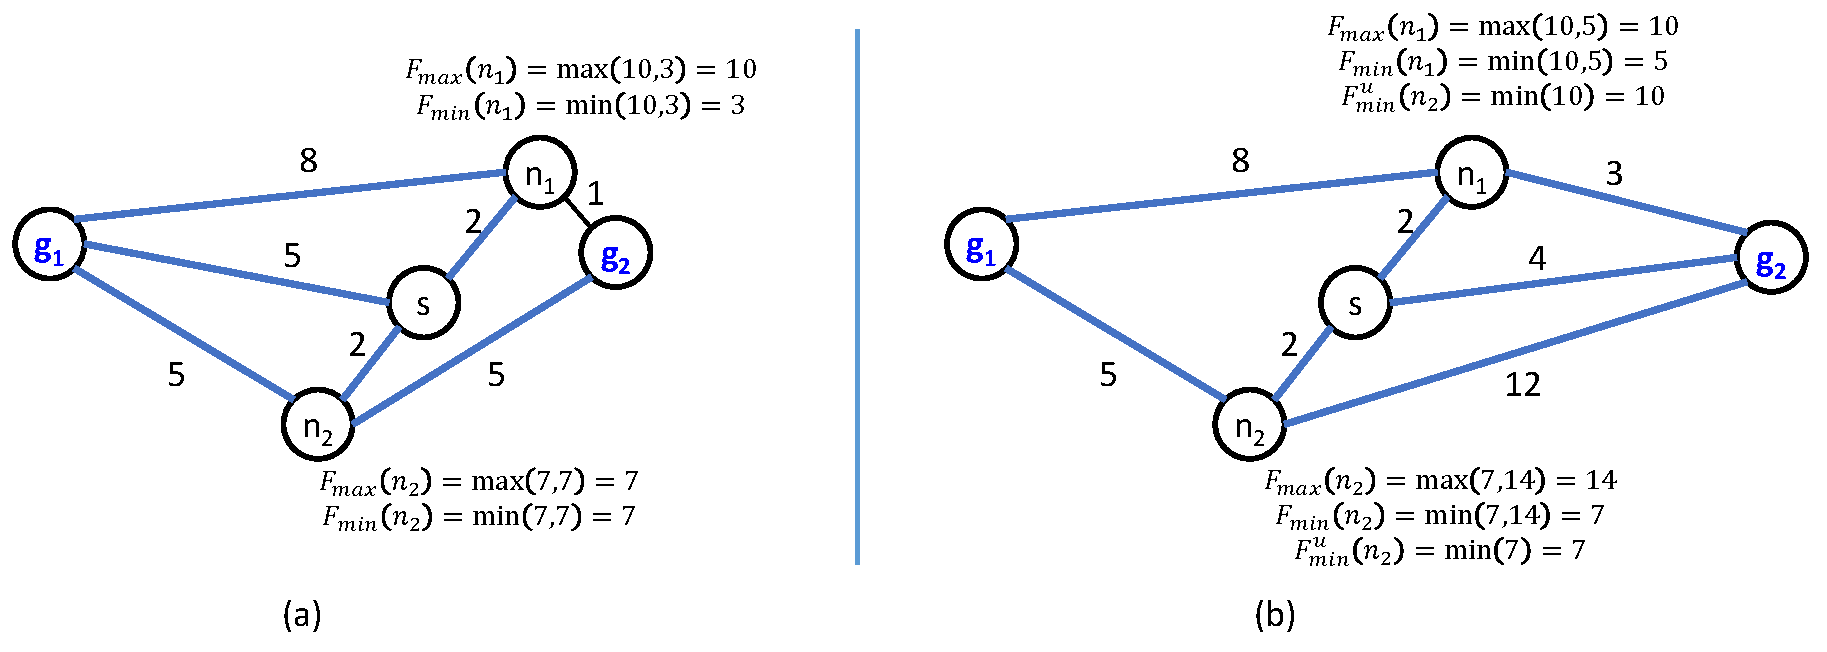
\includegraphics[width=\textwidth]{Lazy_cropped.pdf}      
	\caption{The left hand graph shows an example where using \maxf{} with Lazy \kastar{} results in suboptimal solutions. The right hand graph shows a similar example, but where using Lazy \kastar{} does result in an optimal solutions.}
	\label{fig:lazy}
\end{figure*}

As an example, consider running Lazy \kastarmin{} on the graph depicted in the right hand side of Figure~\ref{fig:lazy}. Assume we have a perfect heuristic in all states except for the goal states $g_1$ and $g_2$ that have a zero heuristic to each other, i.e., $h_2(g_1)=0$ and $h_1(g_2)=0$. After expanding the start state $s$, states $n_1$, $n_2$, and $g_2$ are generated. Using \minf{}, we have $F(n_1)=\min(10,5)=5$, $F(n_2)=\min(7,14)=7$, and $F(g_2)=\min(0,0)=0$. So the next state expanded is goal $g_2$, which is then removed from the set of active goals. At this stage, states $n_1$ and $n_2$ are both in \open{} and their $F$ values are {\em stale} in the sense that they were computed for $g_1$ and $g_2$ while the set of active goals at this stage contain only $g_2$. According to these stale $F$ values, the next state to choose from \open{} is $n_1$ with $F(n_1)=5$. After popping $n_1$ out of \open{}, however, its $F$ value is re-computed  using Lazy \kastar{}. We denote by $F^u_{min}(n)$ this updated $F$ value of $n$, which is computed with respect to the current set of active goals. According to Lazy \kastar{}, if $F^u_{min}(n)\geq F(n)$ then we set $F(n)$ to be $F^u_{min}(n)$ and re-insert $n$ into \open{}. Consequently, $n_2$ will be expanded, followed by $g_1$, finally finding the optimal path to $g_1$ as well. 


% Lazy does not work for Max-f, but does work on Min-f
\subsubsection{The Correctness of Lazy \kastarmin{}}
The correctness of Lazy \kastar{} depends on the state evaluation function. For example, consider running Lazy \kastarmax{} on the graph in left hand side of Figure~\ref{fig:lazy}. This is a \kgs{} problem with two goals ($k=2$) that is similar to the example discussed above, and we assume here too that we have the perfect heuristic in all states except for the goal states $g_1$ and $g_2$ that has a zero heuristic to each other ($h_2(g_1)=h_1(g_2)=0$). After expanding the start state $s$, states $n_1$, $n_2$, and $g_1$ are generated. Using \maxf{}, we have $F(n_1)=\max(10,3)=10$, $F(n_2)=\max(7,7)=7$, and $F(g_1)=\max(0,0)=0$. Therefore, $g_1$ is expanded, and is subsequently removed from the set of active goals. At this stage, states $n_1$ and $n_2$ are both in \open{} and their $F$ values are {\em stale} in the sense that they were computed for $g_1$ and $g_2$ while the set of active goals at this stage contain only $g_2$. According to these stale $F$ values, the next state to expand is $n_2$ with $F(n_2)=7$. This would result in adding $g_2$ to \open{} with $F(g_n)=7$ and subsequently $g_2$ will be expanded and the search will halt, returning a suboptimal path to $g_2$ through $n_2$. If, after $g_1$ was removed from the set of active goals the $F$ values of the states in \open{} would have been re-computed and \open{} re-sorted accordingly, then $n_1$ would have been expanded before $n_2$, finding the optimal path to $g_2$. Thus, {\bf using Lazy \kastarmax{} is not correct, potentially leading to suboptimal paths to some of the goals}. By contrast, Lazy \kastarmin{} is correct, as we show next. 


% Lazy with minf is good
\begin{theorem}[Lazy \kastarmin{} is admissible]
Every path $\pi_i$ returned by Lazy \kastarmin{} with is guaranteed to be the lowest-cost path to its corresponding goal ($g_i$).
\label{the:lazy-minf-correct}
\end{theorem}
\begin{proof}
	We prove Theorem~\ref{the:lazy-minf-correct} by showing that Lazy \kastarmin{} and \kastarmin{}  expand exactly the same set of states. For every $n$ it holds that $F_{min}(n)\leq F^u_{min}(n)$, since $F^u_{min}(n)$ is the minimum over a subset of elements that $F_{min}(n)$ is a minimum of. 
	Since it was chosen for expansion then $n$ has the smallest $F$ value in \open{}
	and $F_{min}(n)=F^u_{min}(n)$, i.e., its $F$ value is not stale, as otherwise it would have been re-inserted into \open{}. Therefore 
	\[ \forall n'\in\open{} ~~ F^u_{min}(n)=F_{min}(n)\leq F_{min}(n') \leq F^u_{min}(n') \]
	So, $n$ has the smallest $F^i_{min}$ value in \open{}, and thus it would have also been expanded by \kastar{}. 
\end{proof}
[[AF: The proof is hard to follow. We can talk and see]]
	


%Of course, one may still use Max-$f$ as an anytime algorithm.  Instead of assuming that when expanding a goal the best path to it has been found, we continue the search, , still looking for better path to that goal. The search halted when [[Roni: do we still need to compute the heuristic for these goals?]] [[Roni: What is a good stopping condition for this option?]]
%Concretely, we continued to compute the heuristic for all goals even after they were expanded, thus continuing to guide the search to look for better path continuing the search and looking for better path to the previously expanded goals. 

\section{Theoretical Analysis}
% Analysis
In this section we compare analytically the two main approaches we proposed for the \kgs{} problem: $k$ searches for one goal (\kxastar{}) or one search for $k$-goals (\kastar{}). 

\subsection{Expanded States and Memory Requirements}
First, we analyze the set of states expanded by the two approaches.  
We denote by Exp(\astari{i}), Exp(\kxastar{}), Exp(\kastarmin), and Exp(\kastarmax), 
the set of states expanded by \astari{i} (for a given $i$), \kxastar{}, \kastarmin, and \kastarmax{}, respectively. It is easy to see that
\[ Exp(\text{\kxastar{}})=\cup_{i=1}^k Exp(\text{\astari{i}}) \]
 
The relation between Exp(\kxastar{}), Exp(\kastarmin), and Exp(\kastarmax) is given in the following observation.
\begin{observation}
	\kastarmin{} expands exactly the same set of states as \kxastar{}, 
	and \kastarmax{} expands all these states and possibly more. Formally:
	\begin{enumerate}
		\item Exp(\kastarmin{})=Exp(\kxastar{})
		\item Exp(\kastarmax{})$\supseteq$ Exp(\kxastar{})
	\end{enumerate}
\label{obs:expandedStates}
\end{observation}
\roni{Do we need a proof or is it trivial?}

% MAX not optimally effective
Note that there are cases where \kastarmax{} indeed expands surplus states, i.e., cases where the set of states expanded by \kastarmax{} is a strict superset of the set of states expanded by \kxastar{}. 
For example, if there are two goals $g_1$ and $g_2$, and three states in \open{} $A$, $B$, and $C$, 
such that ${\bf h}(A)=(2,9)$, ${\bf h}(B)=(9,2)$, and ${\bf h}(C)=(5,5)$. The optimal path may be found without expanding $C$, but using \maxf{} we will choose $C$ before $A$ and $B$. 


% Memory=generated
The number of states expanded is directly related to the number of generated states,
which in turn is related to the memory requirements of \astar{} and \kastar{}. 
In general, best-first search algorithms list \astar{} and \kastar{} are known to be memory intensive, 
storing the states in \open{} and in \closed{} to be able to perform duplicate detection 
and to choose the best state from \open{}. 
While other implementations are also possible, where only the states in \open{} and their predecessors are stored~\cite{zhou2006breadth,korf2004best} or where the states are stored in external memory~\cite{zhou2004structured,edelkamp2016external,edelkamp2005external}, we focus our analysis on the more common implementation of \astar{} in which all generated states are stored in-memory for the entire duration of the search. 
Hence, the memory required for the algorithms discussed in this paper proportional to the number of (distinct) states generated times the memory required to store a single states. %Without loss of generality, assume that each state requires one memory units to store and denote by Gen($X$) the set of states generated by algorithm $X$. From Observation~\ref{obs:expandedStates}, we can bound the memory required to run \kastarmin{} as follows:  
In our analysis we make the simplifying assumption that each state requires one memory unit to store for all algorithms. 
\footnote{This assumption is not exactly correct in practice, since in \kastar{} we store for a state a vector of $k$ values ($\textbf{f}(n)=(f_1,\ldots,f_k)$)  while in \astar{} we only store a single value. Nonetheless, we justify our assumption for cases where the memory required to store the state details is significantly larger than these $k$ values.} 
Hence, if Mem($X$) and Gen($X$) denotes the memory required and the of states generated when running algorithm $X$, respectively, then:
\begin{align}
Mem(\text{\kxastar{}})&=\max_{j\in [1,k]}| Gen(\text{\astari{j}})| \label{eq:kxastar-mem}\\
Mem(\text{\kastarmin{}})&=|\bigcup_{j\in [1,k]} Gen(\text{\astari{j}})| \label{eq:kastar-mem}\\
Mem(\text{\kxastar{}})&\leq Mem(\text{\kastarmin{}}) \leq \sum_{j\in[1,k]} Mem(\text{\astari{j}}) \label{eq:kxastar-kastar-mem}
\end{align}
The correctness of Equations~\ref{eq:kxastar-mem}-\ref{eq:kxastar-kastar-mem} is now explained. 
Since \kxastar{} runs the $k$ searches individually, there is no need to store the states generated by \astari{i} when running \astari{j}. Thus, to run \kxastar{} we require memory sufficient to run each \astari{i} individually (Equation~\ref{eq:kxastar-mem}). In \kastarmin{} we expand the same set of states as \kxastar{} and thus generate the same set of states, but we must store them throughout the search. Thus, \kastar{} stores every state $n$ that is  generated by one of the $k$ searches in \kxastar{}, i.e., the union $\bigcup_{j\in[1,k}Gen(\astari{j}$ (Equation~\ref{eq:kastar-mem}). The size of this union cannot be smaller than the cardinality of the set of stated generated by any individual \astar{}, but cannot be larger than their sum (Equations~\ref{eq:kxastar-kastar-mem}). Note that these bounds are tight, in the sense that there are \kgs{} problems where 
$Mem(\text{\kxastar{}}) = Mem(\text{\kastarmin{}})$ and other \kgs{} problems where 
$Mem(\text{\kastarmin{}}) = \sum_{j\in[1,k]} Mem(\text{\astari{j}})$. 



\subsection{Runtime Analysis}
Now we analyze the expected runtime of the proposed \kgs{} algorithms. As shown above theoretically 
and will be showed later experimenally, \kastarmin{} is almost always superior to \kastarmax{}, 
and thus the focus of our analysis is a comparison between \kxastar{} and \kastarmin{}. 
While both algorithms generate the same set of states (Observation~\ref{obs:expandedStates}), 
their runtime differ due to the number of times each state is generated and the cost of these generations. 
Let Time($X$) be the running time required for algorithm $X$. 
Computing Time(\kxastar{}) is straightforward: every $k$ search is done independently, incurring a cost of $C_{gen}+C_{dd}+C_h+C_{add}$ per generated states. 
\[ 
Time(\text{\kxastar{}}) = \sum_{i\in[1,k]} |Gen(\text{\astari{i}})|\cdot (C_{gen}+C_{dd}+C_h+C_{add})
\]

For \kastar{}, a deeper analysis is needed. Consider the number of times each of the costs components -- $C_{gen}$, $C_{dd}$, $C_h$, and $C_{add}$ -- is incurred.\\
{\bf $\mathbf{C_{gen}}$ and $\mathbf{C_{dd}}$.} Every generated state incurs $C_{gen}$ and $C_{dd}$ exactly once. 
Thus, state generation and duplicate detection add to the overall running time:
\[ 
|\bigcup_{i\in{1,k}} Gen(\text{\astari{i}})|\cdot (C_{gen}+C_{dd}) = Gen_k(k)\cdot (C_{gen}+C_{dd}) 
\displaystyle
\]
$\mathbf{C_{h}}.$ Without loss of generality, assume that $g_1$ is the goal expanded first by \kastarmin{}, 
then $g_2$, and so on, until $g_k$ is last goal that is expanded (after which the search halts). 
Until the first goal is expanded, \kastar{} computes $k$ heuristics, 
then, until the second is expanded, \kastar{} computes $k-1$ heuristics, and so on. 
So, $Gen_k(1)$ states are generated with $k$ heuristics, 
$Gen_{k}(2)$ states with $k-1$ heuristics,a nd so on. Summing all this, we have that 
in \kastarmin{}, heuristic computations add to the overall running time:
\[ \sum_{i\in[1,k]} Gen_k(i)\cdot C_h \]

$\mathbf{C_{add}}.$ Every generated state is added at least once, 
incurring $C_{add}\cdot |Gen(\text{\kastar{}})|=C_{add}\cdot Gen_k(k)$. 
In addition, \open{} gets re-sorted after every goal is found (except for the last goal). 
Re-sorting \open{} constitutes iterating over all the states in it and adding them again (with a corrected $F$ value). 
The corresponding computational cost is the number of states in \open{} times $C_{add}$. 
So, if $O_i$ is the number of states in \open{} when goal $g_i$ is expanded, then 
the cost added to the overall running time that is due to adding states to \open{} is:
\[ Gen_k(k)+\sum_{i\in[1,k-1]} O_i \]

\begin{table}
	\begin{tabular}{|l|l|l|}
		\hline
		Cost 		& \kxastar{}									& \kastarmin \\ \hline
		$C_{gen}$	& $\sum_{i\in[1,k]} |Gen(\text{\astari{i}})|$		& * $|\bigcup_{i\in[1,k]} Gen(\text{\astari{i}})|$\\
		$C_{dd}$	& $\sum_{i\in[1,k]} |Gen(\text{\astari{i}})|$		& * $|\bigcup_{i\in[1,k]} Gen(\text{\astari{i}})|$\\
		$C_{h}$		& * $\sum_{i\in[1,k]} |Gen(\text{\astari{i}})|$		& $\sum_{i\in[1,k]} Gen_k(i)$\\
		$C_{add}$	& $\sum_{i\in[1,k]} |Gen(\text{\astari{i}})|$		& $|\bigcup_{i\in[1,k]} Gen(\text{\astari{i}})|
		+ \sum_{i\in[1,k-1]} O_i$ \\			
		\hline		
	\end{tabular}
	\caption{Analysis of the computational costs incurred by \kxastar{} and \kastarmin{} 
		when solving a \kgs{} problem with arbitrary $k$. 
		Some costs are incurred the same or less in one algorithm than the other. Such cases are marked with an asterisk. }
	\label{tab:time-analysis}	
\end{table}

Table~\ref{tab:time-analysis} summarizes the above analysis, comparing 
the running times of \kxastar{} and \kastarmin{}. Each row represents one of the computational costs factors ($C_{gen}$, $C_{dd}$, $C_{h}$, and $C_{add}$), showing the contribution of that computational cost factor to the overall running time for the compared algorithms. To show the usefulness of the above analysis, we consider some special cases.
\begin{itemize}
	\item {\bf Case 1: State generation costs is dominant.} ($C_{gen}>>C_{dd}+C_{h}+C_{add}$) 
	If this case, the preferred algorithm is \kastar{}. To show this, 
	compare the values in Table~\ref{tab:time-analysis} for $C_{gen}$: $\sum_{i\in[1,k]} |Gen(\text{\astari{i}})|$ 
	versus $|\bigcup_{i\in[1,k]} Gen(\text{\astari{i}})|$. Clearly, the former is larger than or equal to the latter. 
	How large the advantage of \kastarmin{} is will depend on the size of the intersection between the sets $Gen(\text{\astari{i}})$ for $i\in[1,k]$. 
	
	\item {\bf Case 2: Heuristic computation is dominant.} ($C_{h}>>C_{gen}+C_{dd}+C_{add}$) 
	If this is the case, the preferred algorithm is \kxastar{}. Again, to show this we look to Table~\ref{tab:time-analysis} and see that \kxastar{} computes a heuristic function  
	$\sum_{i\in[1,k]} |Gen(\text{\astari{i}})|$ times, while 
	\kastar{} computes the heuristic $\sum_{i\in[1,k]} Gen_k(i)$ times. 
	Importantly, for every $i$ it holds that $Gen_k(i)\geq |Gen(\text{\astari{i}})|$
	because $Gen_k(i)$ counts all the states in $Gen(\text{\astari{i}})$ 
	and states from other searches that happen to have been added to \open{} at this stage. 		
\end{itemize}

\roni{Do we need the 2-goal illustration? I have text for it in the drafts.tex}
\section{Experimental Results}

%In this section we compared empirically the performance of the four \kgs{} algorithms we discussed: $k$ \astar{} searches (Section~\ref{sec:k-one-goal}), two versions of \kastar{} (Section~\ref{sec:one-k-goal-search}): \kastarmax{} and \kastarmin{}, and Lazy \kastar{} with \minf{} (Section~\ref{sec:lazy}). We also compared these heuristic search algorithms with uniform cost search. 


In this section we compared empirically the performance of the four \kgs{}
algorithms we discussed: 
\kxastar{} (Section~\ref{sec:k-one-goal}), 
\kastarmax{} and \kastarmin{}(Section~\ref{sec:one-k-goal-search}),  
and Lazy \kastarmin{}. A fifth algorithm is {\em uniform cost search} (UCS) (also known
as Dijkstra's algorithm) which is a best first search without a heuristic,
i.e., it prioritize nodes based on their $g$ values only.


We evaluated these algorithms on two domains: the pancake puzzle and path finding in grids from the Dragon Age video game from the movingai repository~\cite{sturtevant2012benchmarks}. These two domains represent different types of search problems. The pancake puzzle is an {\em exponential domain}, i.e., the state space graph is exponential in the size of the state, and is given implicitly by a start state and a set of state transition operators. The grid pathfinding domain is a {\em polynomial domain}, i.e., the entire state space graph is given as input, and so the running time of a single path finding search is polynomial in the problem input (the graph). 

\roni{Meir, please add here details about the maps: which map did you use, etc.}
\subsection{Grid Path Finding}
\roni{Meir: what was the heuristic used? how were the states generated? how many instances?}

\begin{table}[]
    \centering
    \begin{tabular}{|r|r|r|r|r|r|}
    \hline
        & \multicolumn{1}{c|}{Lazy \kastarmin{}} & \kastarmax &      \kastarmin       &  \kxastar & UCS       \\

        \hline
1     & \textbf{1.9}                 & \textbf{1.9} & \textbf{1.9} & \textbf{1.9} & 3.5          \\
2     & \textbf{3.0}                 & 3.9          & \textbf{3.0} & 3.6          & 4.5          \\
4     & \textbf{4.0}                 & 5.7          & \textbf{4.0} & 6.9          & 5.2          \\
8     & \textbf{5.4}                 & 7.1          & 5.5          & 13.4         & 5.7          \\
16    & 7.0                          & 8.8          & 7.3          & 27.0         & \textbf{6.0} \\
32    & 9.1                          & 10.9         & 10.4         & 54.0         & \textbf{6.2} \\
64    & 12.5                         & 17.1         & 19.3         & 108.9        & \textbf{6.6} \\
128   & 20.5                         & 26.8         & 52.7         & 214.9 &
\textbf{6.7}\\
\hline
    \end{tabular}
    \caption{Running time (in ms.) spent when solving \kgs{} problems with different number of goals ($k$) on the grid pathfinding domain. Highlighted in bold are the best results for every $k$.}
    \label{tab:pathfinding-runtime}
\end{table}

In this domain we performed two type of experiments. In the first type of experiment, the goals were chosen randomly from the set of possible locations in the grid, and we investigated the impact of increasing the number of goals. The results are given in Table~\ref{tab:pathfinding-runtime}. The best results for every $k$ are highlighted in bold. There are several interesting trends to observe here. First, we clearly see that Lazy \kastarmin{} dominates both \kastarmin{} and \kastarmax{}. Second, we see that for every $k>1$, all version of \kastar{} outperforms \kxastar{}. Third, we see that as the number of goals becomes very large, UCS becomes the best algorithm. To explain this, consider the most extreme case, where we every state is a goal. In this case, clearly UCS will be the most effective, as it will expand every state at most once and will never spend any time on computing a heuristic value. By contrast, \astar{} and \kastar{} will compute at least one heuristic for every state, and most likely will compute even more heuristics per state. This heuristic computation time is not spent by UCS. Thus, as we see in the results the benefit of using a heuristic diminishes as the number of goals increase, resulting in UCS outperforming all other searches. 



% Generated states.

\begin{table}[]
    \centering
    \begin{tabular}{|r|r|r|r|r|r|}
    \hline
        & \multicolumn{1}{c|}{Lazy \kastarmin{}} & \kastarmax &      \kastarmin       &  \kxastar & UCS       \\

        \hline
1                         & \textbf{13,987}                      & \textbf{13,987}           & \textbf{13,987}           & \textbf{13,987}                 & 41,122                      \\
2                         & 29,286                               & \textbf{21,682}           & 21,686                    & 27,389                          & 53,583                      \\
4                         & 43,291                               & \textbf{28,413}           & 28,424                    & 52,375                          & 62,826                      \\
8                         & 55,652                               & \textbf{36,650}           & 36,673                    & 101,103                         & 68,505                      \\
16                        & 64,805                               & \textbf{43,489}           & 43,531                    & 202,715                         & 72,196                      \\
32                        & 70,519                               & \textbf{49,662}           & 49,732                    & 407,221                         & 74,618                      \\
64                        & 73,841                               & \textbf{54,239}           & 54,357                    & 823,018                         & 75,998                      \\
128                       & 75,341                               & \textbf{57,739}           & 57,932                    & 1,613,628                       & 76,495\\
\hline
    \end{tabular}
    \caption{The number of states generated when solving \kgs{} problems with different number of goals ($k$) on the grid pathfinding domain. Highlighted in bold are the best results for every $k$.}
    \label{tab:pathfinding-generated}
\end{table}


%\begin{figure}
%	\includegraphics[width=0.45\columnwidth]{Capture-minf.PNG}      
%	\includegraphics[width=0.45\columnwidth]{Capture-maxf.PNG}      
%	\caption{XXx}
%	\label{fig:min-vs-max}
%\end{figure}

\begin{figure}
	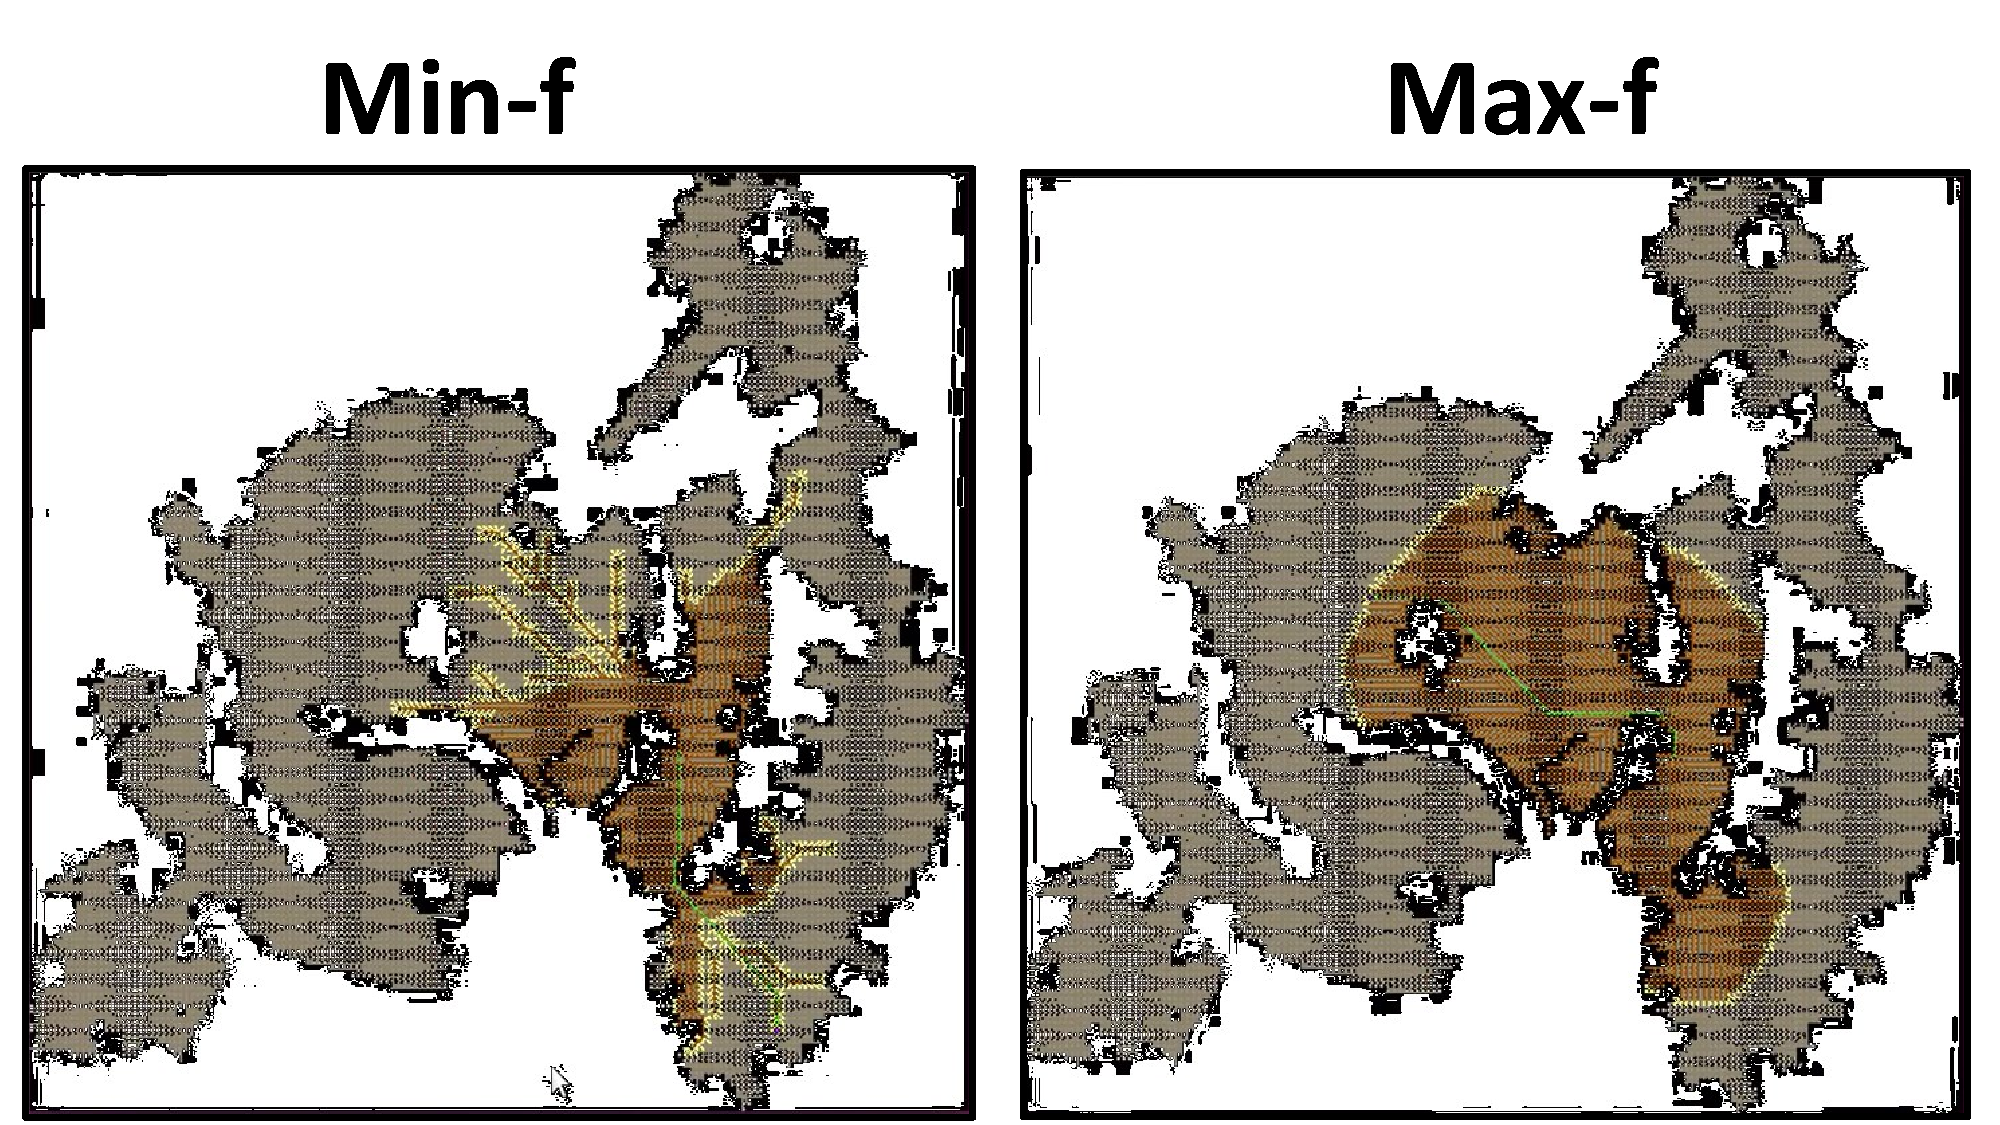
\includegraphics[width=\columnwidth]{min-vs-max}      
	\caption{An example of running \kastar{} with \minf{} (left) and with \maxf{} (right). The yellow parts represent the states in \open{}, the brown parts represent the states in \closed{}.}
	\label{fig:min-vs-max}
\end{figure}

To provide a deeper insight, Table~\ref{tab:pathfinding-generated} shows the average number of states generated for each algorithm until it halts. Here too we highlihgted the best results for every $k$ in bold. 
First, observe that even when the number of goals is large, uniform cost search generates more states than than the \kastar{} variants. This confirms our explanation above: when the number of goals is large, the  runtime of uniform cost search was lower than all other algorithm not because it generated fewer states, but because its time per state is smaller (due to not needing to compute heuristics). 

Second, the number of states generated by \kastarmax{} is slightly smaller than that of \kastarmin{}. To explain this, consider the illustrations in Figure~\ref{fig:min-vs-max}. They show an example of running \kastarmin{} (left) and \kastarmax{} (right) on the same \kgs{} instance. The yellow points represent states in \open{}, the brown points represent states in \closed{}, the graph points are states that were not generated so far and the yellow points are impassable obstacles. As can be seen, the behavior of \kastarmin{} and \kastarmax{} are different: \kastarmin{} runs greedily towards prospective goals, showing clear trajectories protruding from the search frontier, while \kastarmax{} demonstrates a behavior that is more similar to uniform cost search. This is reasonable, because when in \kastarmin{} a child that is generated that is closer to the closest goal of its parent will expanded next, resulting in these protruding trajectories towards the goal. By contrast, in \kastarmax{} even if a state generates a child state that is closer to the closest goal, it still may not be expanded because it is further from some other goal. \roni{Probably there's a nicer way to explain this.} 
[[AF: Yes there	is. We need to think]]
This behavior results in \kastarmin{} having a weaker duplicate detection phase compared to \kastarmax{}, resulting in a bigger \open{} and thus more generated states. 

\roni{Can anyone explain why Lazy \kastar{} generates more states?}
[[AF: Lazy should be identical to \kastarmin{}. Maybe they had different tie breaking?]]




\begin{figure}
	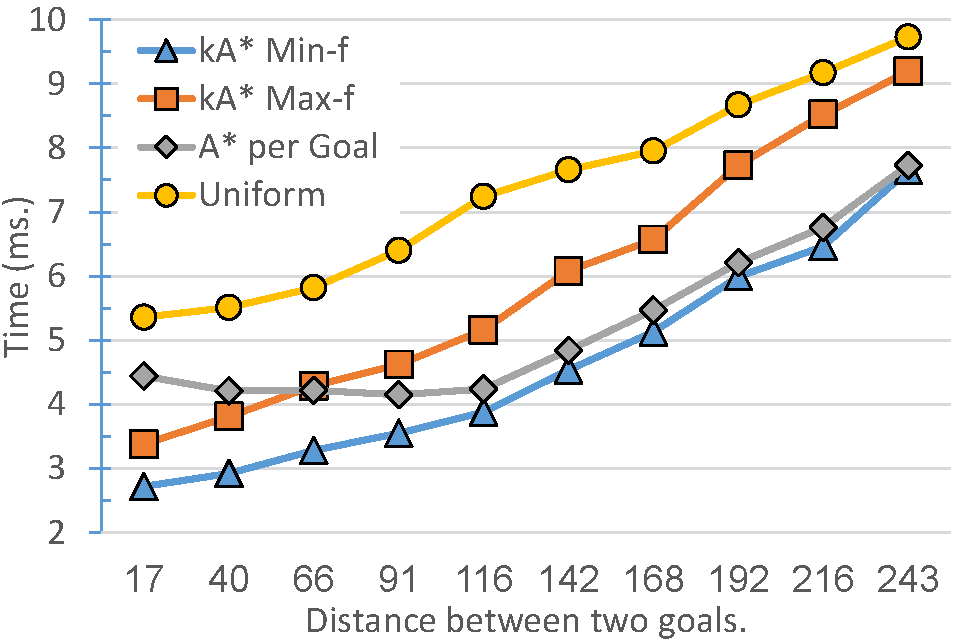
\includegraphics[width=\columnwidth]{G0-G1_cropped.pdf}      
	\caption{This figure plots the runtime (in ms.) of the different \kgs{} algorithms as a function of the distance between the goals, for a \kgs{} problem with two goals ($k=2$).}
	\label{fig:2-goal}
\end{figure}
In the second type of experiments we performed, we focused on \kgs{} problems with two goals ($k=2$), and investigated the impact of the distance between these goals on the effectiveness of the evaluated algorithms. 
The results are given in Figure~\ref{fig:2-goal}. The $x$-axis is the distance between the goals, and the $y$-axis shows the average runtime in milliseconds of the different algorithms. 
\roni{Meir, is this Lazy \kastarmin{} or regular \kastarmin{}?} 
We observe several trends. 
First, for a 2 goal problem it is clear that uniform cost search is the worst option. 
This is reasonable, as it does not use a heuristic to guide its search and the number of goals is small. 
Second, observe that when the goals are close to each other, both \kastarmin{} 
and \kastarmax{} outperform \kxastar{}. This matches our analytical analysis, where if the goals are close to each other we expect that there will be many states that will be expanded by both independent \astar{} searches, introducing exactly the redundancy \kastar{} was designed to solve. 
Following this explanation, we observe that as the goals chosen become further from each other (going right on the $x$ axis of Figure~\ref{fig:2-goal}), we see the advantage of \kastar{} over 2 \astar{} searches diminishes. Indeed, the performance of \kastarmin{}  and \kxastar{} converge when the goals are furthest from each other. 
Lastly, we observe that \kastarmin{} dominates \kastarmax{} and in general all other approaches, always being better or on par with the other algorithms. 



\subsection{Pancake Puzzle}

\begin{table}[]
    \centering
    \begin{tabular}{|r|r|r|r|r|}
	\hline
        \multicolumn{1}{|l|}{}            & \multicolumn{2}{c|}{Runtime (ms.)}                                       & \multicolumn{2}{c|}{Generated} \\ \hline
        \multicolumn{1}{|c|}{\# Pancakes} & \multicolumn{1}{c}{\kastarmax{}} & \multicolumn{1}{c|}{Uniform} & \multicolumn{1}{c}{\kastarmax{}} & \multicolumn{1}{c|}{Uniform} \\ \hline
        6                               & 0.34                                      & 0.46                        & 994                                       & 2,287                       \\
        7                               & 2.57                                      & 4.06                        & 8,617                                     & 21,059                      \\
        8                               & 22.95                                     & 40.25                       & 74,745                                    & 188,946                     \\
        9                               & 410.81                                    & 717.64                      & 787,481                                   &
        1,973,420\\
        \hline
    \end{tabular}
    \caption{Running time (in ms.) and number of generated states for solving \kgs{} with two goals 
    	in the Pancake puzzle domain using UCS and \kastarmax{}.}
\label{tab:pancake-max-uniform}
\end{table}

Next, we present the results for the pancake puzzle. 
\roni{Meir: what was the heuristic used? how were the states generated? how many instances?}
The first results we report is that uniform cost search and \kastarmax{} 
could not solve even small-sized problems even for $k=2$. Average running time and number of states generated  for $k=2$ and pancakes of size up to 9 are given in Table~\ref{tab:pancake-max-uniform}. These results are reasonable because in exponential domains running a search without a heuristic is not practical, and \kastarmax{} can behave similar to uniform cost search (as shown also in Figure~\ref{fig:min-vs-max}). 


\begin{table*}[]

		
		    \centering
		\begin{tabular}{|r|r|r|r|r|r|r|r|r|}
			\hline
			& \multicolumn{4}{c|}{{\bf 10 Pancakes}} & \multicolumn{4}{c|}{{\bf 20 Pancakes}}    \\
			\hline
			& \multicolumn{2}{c|}{Average of Time (ms.)}   & \multicolumn{2}{c|}{Average of Generated}    & \multicolumn{2}{c|}{Average of Time (ms.)}   & \multicolumn{2}{c|}{Average of Generated}    \\
			\hline
			$k$ & \kastarmin{} & \kxastar{} & \kastarmin{} & \kxastar{} & \kastarmin{} & \kxastar{} & \kastarmin{} & \kxastar{}  \\ \hline
		
1           & 0.09                  & \textbf{0.08}       & \textbf{190}          & \textbf{190}        & 4.24                  & \textbf{4.17}       & \textbf{7,324}        & \textbf{7,324}      \\
2           & 0.20                  & \textbf{0.16}       & \textbf{363}          & 368                 & 9.75                  & \textbf{7.81}       & \textbf{13,794}       & 13,828              \\
4           & 0.51                  & \textbf{0.35}       & \textbf{755}          & 788                 & 21.74                 & \textbf{13.73}      & 25,154                & \textbf{24,982}     \\
8           & 1.18                  & \textbf{0.67}       & \textbf{1,364}        & 1,512               & 66.63                 & \textbf{30.14}      & \textbf{53,268}       & 53,790              \\
16          & 3.24                  & \textbf{1.35}       & \textbf{2,645}        & 3,058               & 206.03                & \textbf{59.51}      & \textbf{103,674}       & 105,863     \\ \hline
	\end{tabular}
	\caption{The average runtime and average number of states generated in the pancake experiments, for \kastar{} with \minf{} and for running $k$ independent \astar{} searches. Best results per $k$ are highlighted in bold.}
	\label{tab:pancake-minf-k-searches}
\end{table*}


Table~\ref{tab:pancake-minf-k-searches} presents the results for 10 pancakes and for 20 pancakes, for 1, 2, 4, 8, and 16 goals, comparing \kastarmin{} and \kxastar{}. 
The results show that while \kastarmin{} usually generates fewer states, its overall runtime is comparable or worse than running \kxastar{}. This is because in exponential domains the intersection between the sets of states generated by each search is small compared to size of the last $f$ layer of each search. \roni{Meir and Ariel, I'm looking for a nicer explanation. Any thoughts?}


To conclude our experimental results, we observed the following trends:
\begin{enumerate}
	\item In the pancake domain, running $k$ individual searches (\kxastar{}) is better than \kastar{}, because the overlap of states generated by more than one search is small.
	\item In the grid pathfinding domain, however, many states are generated by more than one search, and consequently \kastar{} is advantageous compared to \kxastar{} searches. 
	\item \kastarmin{} usually outperforms \kastarmax{}, but not always. Lazy \kastar{} outperforms both. 
	\item When the number of goals becomes very large, simply running UCS is the best option, as it does not spend time on heuristic computations. 
\end{enumerate}

\roni{TODO: ADD MORE HERE}




\subsection{Related work}
\label{sec:related-work}

There are several well-studied graph problems that are related to $k$-goal search. In the traveling salesman problem (TSP), we aim to find a shortest path that passes through a set of vertices. 
...

In multi-objective search, we have multiple objectives function that we wish to optimize. E.g., in a navigation application one may want to optimize for path length and also for ease of navigation. An optimal 
solution to a multi-objective optimization problem is usually a solution that is Pareto-optimal, and it is often the case that one would like the set of all Pareto-optimal solutions. 


An important distinction to make is that \kgs\ is different from the problem where $k$ possible goals are given and the task is to find the shortest path to the closest goal. In \kgs\ we must find the shortest path to each of the goals, and not just to the closest one. 


The \kgs{} problem is related to the problem addressed by incremental search algorithms such as Lifelong Planning \astar{}~\cite{koenig2004lifelong}. Incremental search algorithm are designed to solve a sequence of search problems, where the start and goal of these search problems are the same, but the underlying graph has changed. The key idea in incremental search algorithms is to re-use information from previous searches to solve faster the current search problem. However, unlike the incremental search setting is different from \kgs{}: in incremental search we have one goal and the environment is dynamic, while in \kgs{} we have $k$ goals but assume the environment does not change. 

Another related problem is the moving-target search problem. Moving-target search problems are search problems where the goal changes during the search. This is different from \kgs{} where the goals do not change during the search, but we know upfront the $k$ goals. 

\section{Conclusion and Future Work}



In future work we will explore ways in which the search for one goal 
can provide information to help searching for the other goals. 

One way to do so in undirected graphs is to use the heuristic for one goal and the 
heuristic between the goals as an admissible heuristic, thus allowing to save the computational cost of re-computing the heuristic of a state if it is generated again for the other goal. This idea is inspired from the canonical heuristics used by path finding algorithms~\cite{canonical}.



% \begin{figure}[!htbp]
%   \centering
%   \includegraphics[width=1\hsize]{filename.eps}
%   \caption{caption} \label{fig:label}
% \end{figure}

\section*{Acknowledgements}
Thanks!

\bibliographystyle{abbrv}
\bibliography{library}

\end{document}
